\section{Experimental Results and Analysis}
\label{sec:results}
The results quantify model performance exclusively on the held-out 2016--2018 test partition. Table~\ref{tab:model_performance} details the primary evaluation metrics.

\begin{table}[htbp]
\caption{Final Offline Test Performance (2016--2018)}
\begin{center}
\resizebox{\columnwidth}{!}{
\begin{tabular}{l l r r r r r r}
\toprule
\textbf{Hazard} & \textbf{Model} & \textbf{Acc} & \textbf{Prec} & \textbf{Rec} & \textbf{F1} & \textbf{ROC} & \textbf{PR}\\
\midrule
Flood & Random Forest & 0.6916 & 0.3539 & 0.6930 & 0.4686 & 0.7184 & 0.3500 \\
Heatwave & LightGBM & 0.9790 & 0.8558 & 0.9175 & 0.8856 & 0.9966 & 0.9677 \\
Compound & Stacking (Op) & 0.9124 & 0.2960 & 0.8222 & 0.4353 & 0.9553 & 0.4077 \\
Compound & GRU (Offline) & 0.8457 & 0.2010 & 0.9111 & 0.3293 & 0.9423 & 0.2965 \\
\bottomrule
\end{tabular}
}
\label{tab:model_performance}
\end{center}
\end{table}

\subsection{Flood Prediction}
\begin{figure}[!t]
\centering
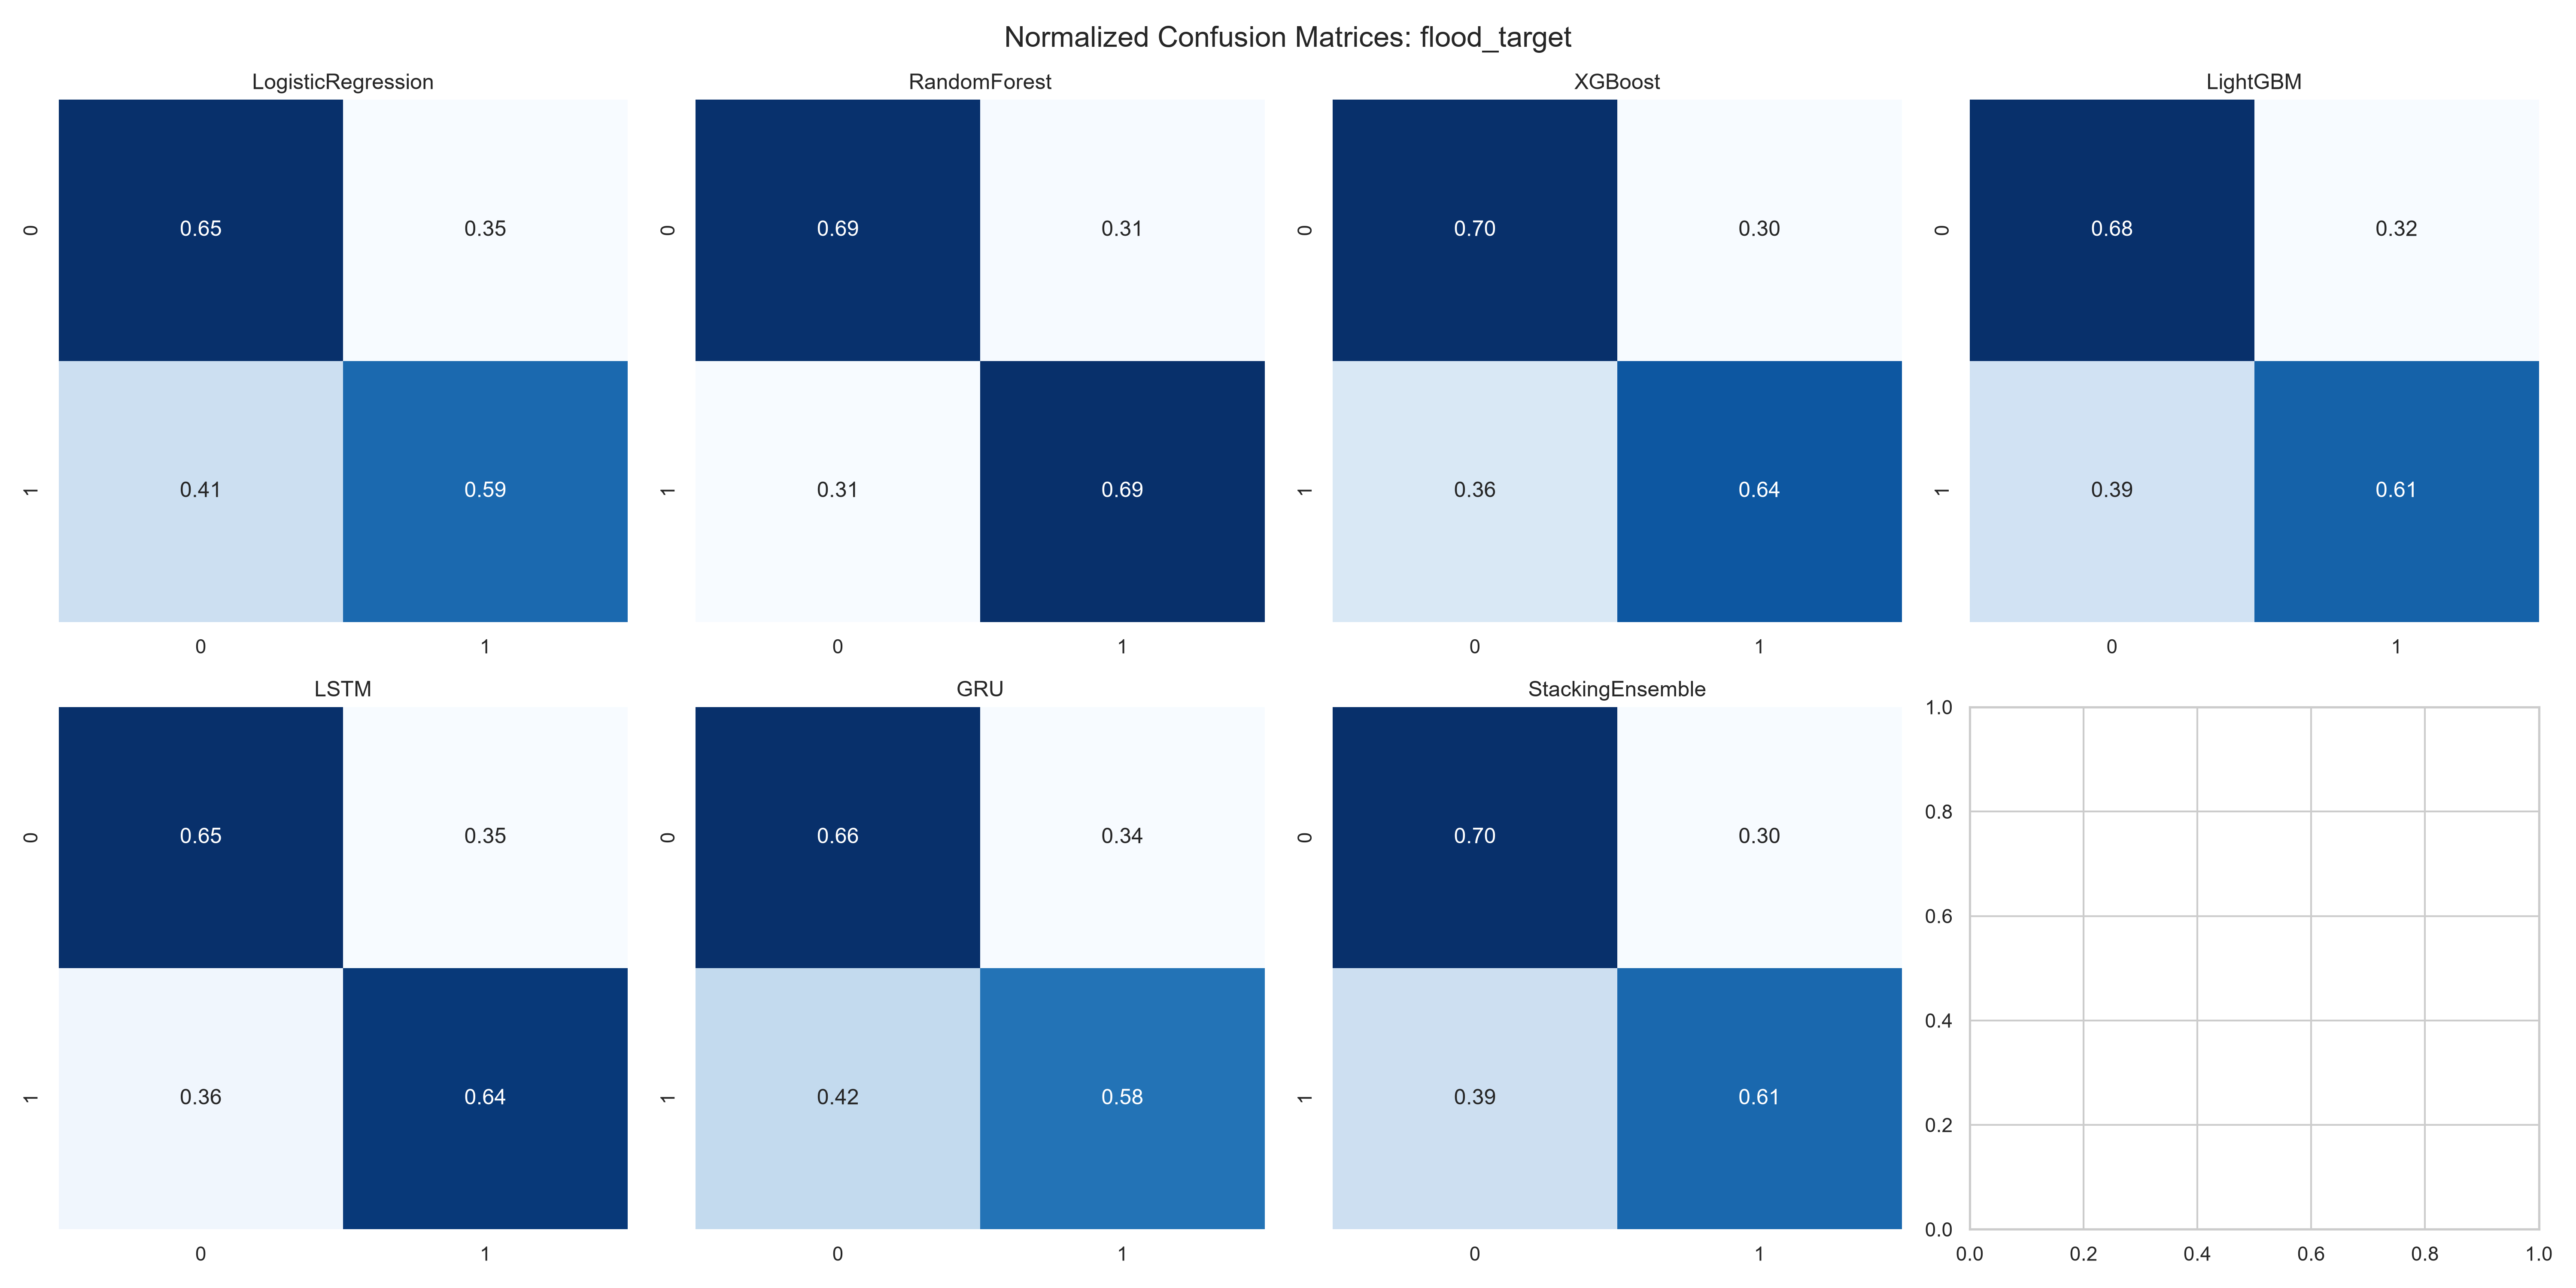
\includegraphics[width=\columnwidth]{../Paper_Figures/Fig_02_Flood_Confusion_Matrix.png}
\caption{Normalized confusion matrix for the flood prediction model on the held-out 2016--2018 test set.}
\label{fig:flood_confusion}
\end{figure}
The Random Forest model demonstrates practical discrimination, achieving an Accuracy of 0.6916, an $F_1$-score of 0.4686, an ROC-AUC of 0.7184, and a Brier Score of 0.2391. The classification mapping (Fig.~\ref{fig:flood_confusion}) highlights the intentional prioritization of Recall (0.6930) over Precision (0.3539), representing an operational trade-off that favors the detection of true emergencies at the cost of elevated false alarms.

\subsection{Heatwave Prediction}
\begin{figure}[!t]
\centering
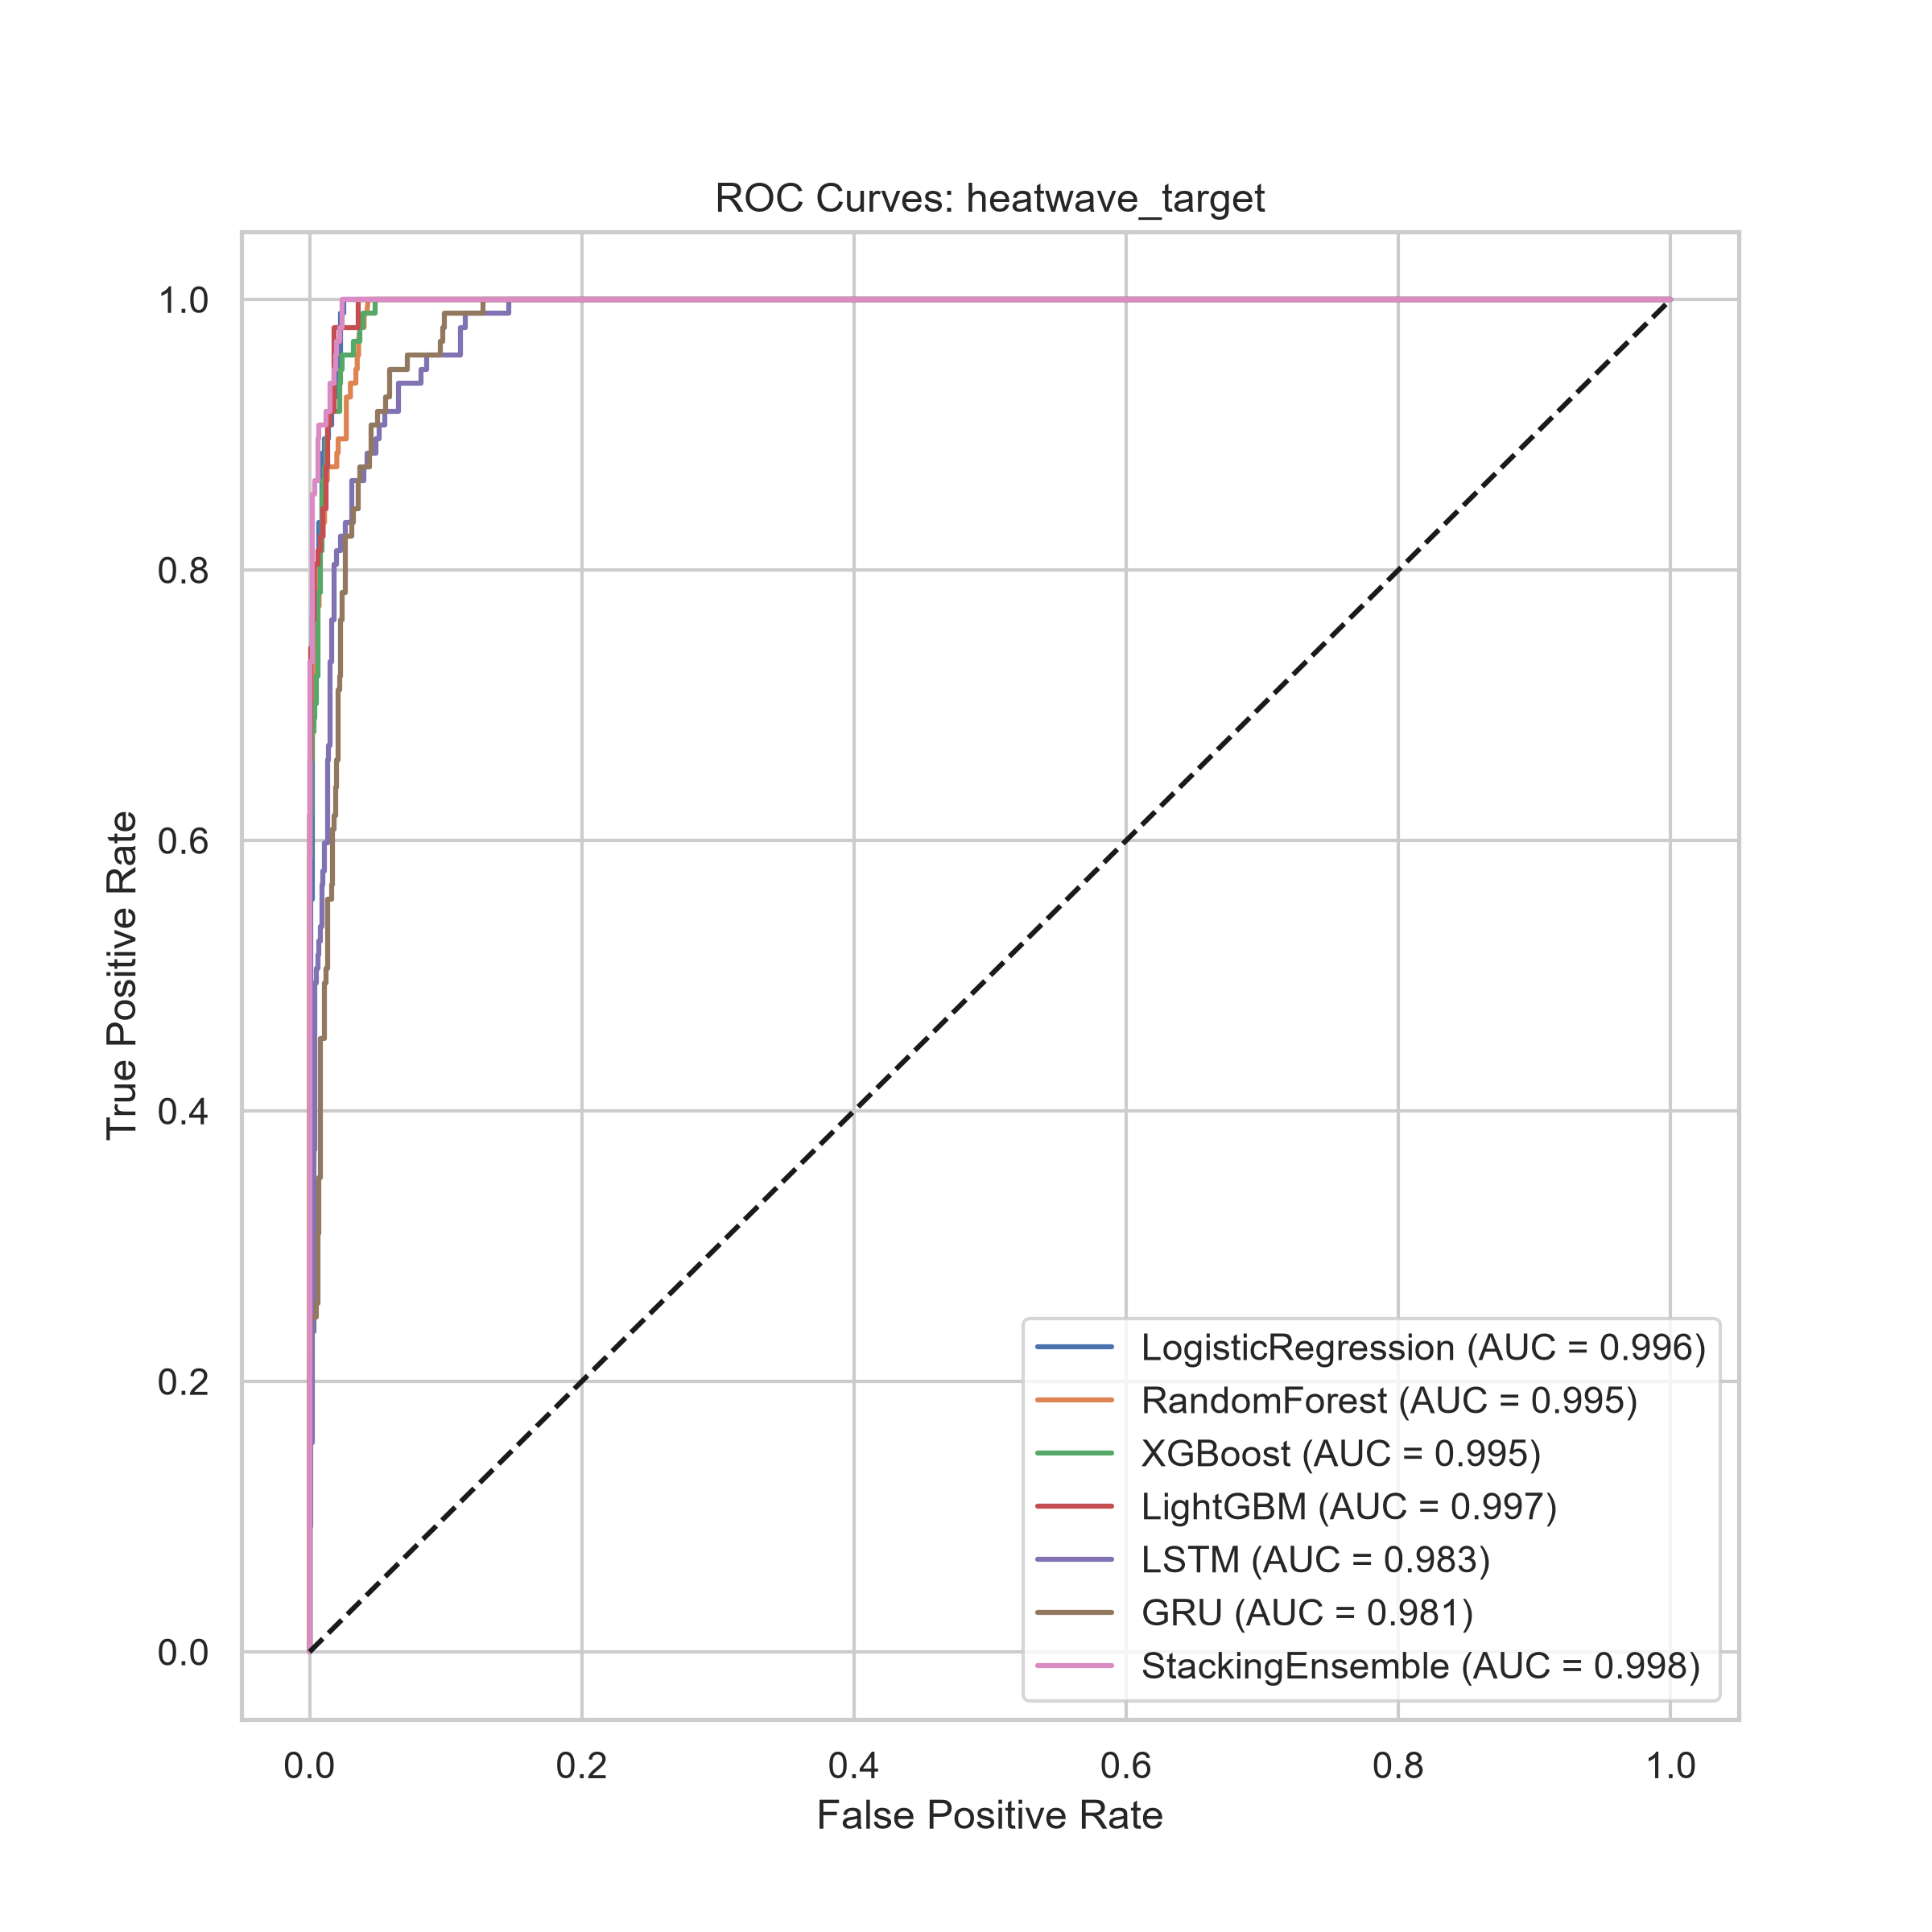
\includegraphics[width=\columnwidth]{../Paper_Figures/Fig_03_Heatwave_ROC.png}
\caption{ROC curve of the heatwave LightGBM classifier on the held-out test set.}
\label{fig:heatwave_roc}
\end{figure}
The proxy-remediated LightGBM classifier achieves extraordinary performance despite operating on a strictly constrained 41-feature subspace. It records an Accuracy of 0.9790, an $F_1$-score of 0.8856, an ROC-AUC of 0.9966, and a highly reliable Brier Score of 0.0159. The corresponding ROC curve (Fig.~\ref{fig:heatwave_roc}) visually affirms this robust boundary definition, confirming that the model effectively maps underlying meteorological drivers without relying on tautological proxy variables.

\subsection{Compound Risk Prediction}
The simultaneous intersection of hazards introduces significant predictive complexity. The operational Stacking Ensemble yields an $F_1$-score of 0.4353 and an ROC-AUC of 0.9553. The GRU sequential benchmark achieved an $F_1$-score of 0.3293 and an ROC-AUC of 0.9423. This confirms that the stateless ensemble architecture outperformed the deep learning sequence benchmark under the evaluated conditions.

\subsection{Lead-Time Analysis}
\begin{figure}[!t]
\centering
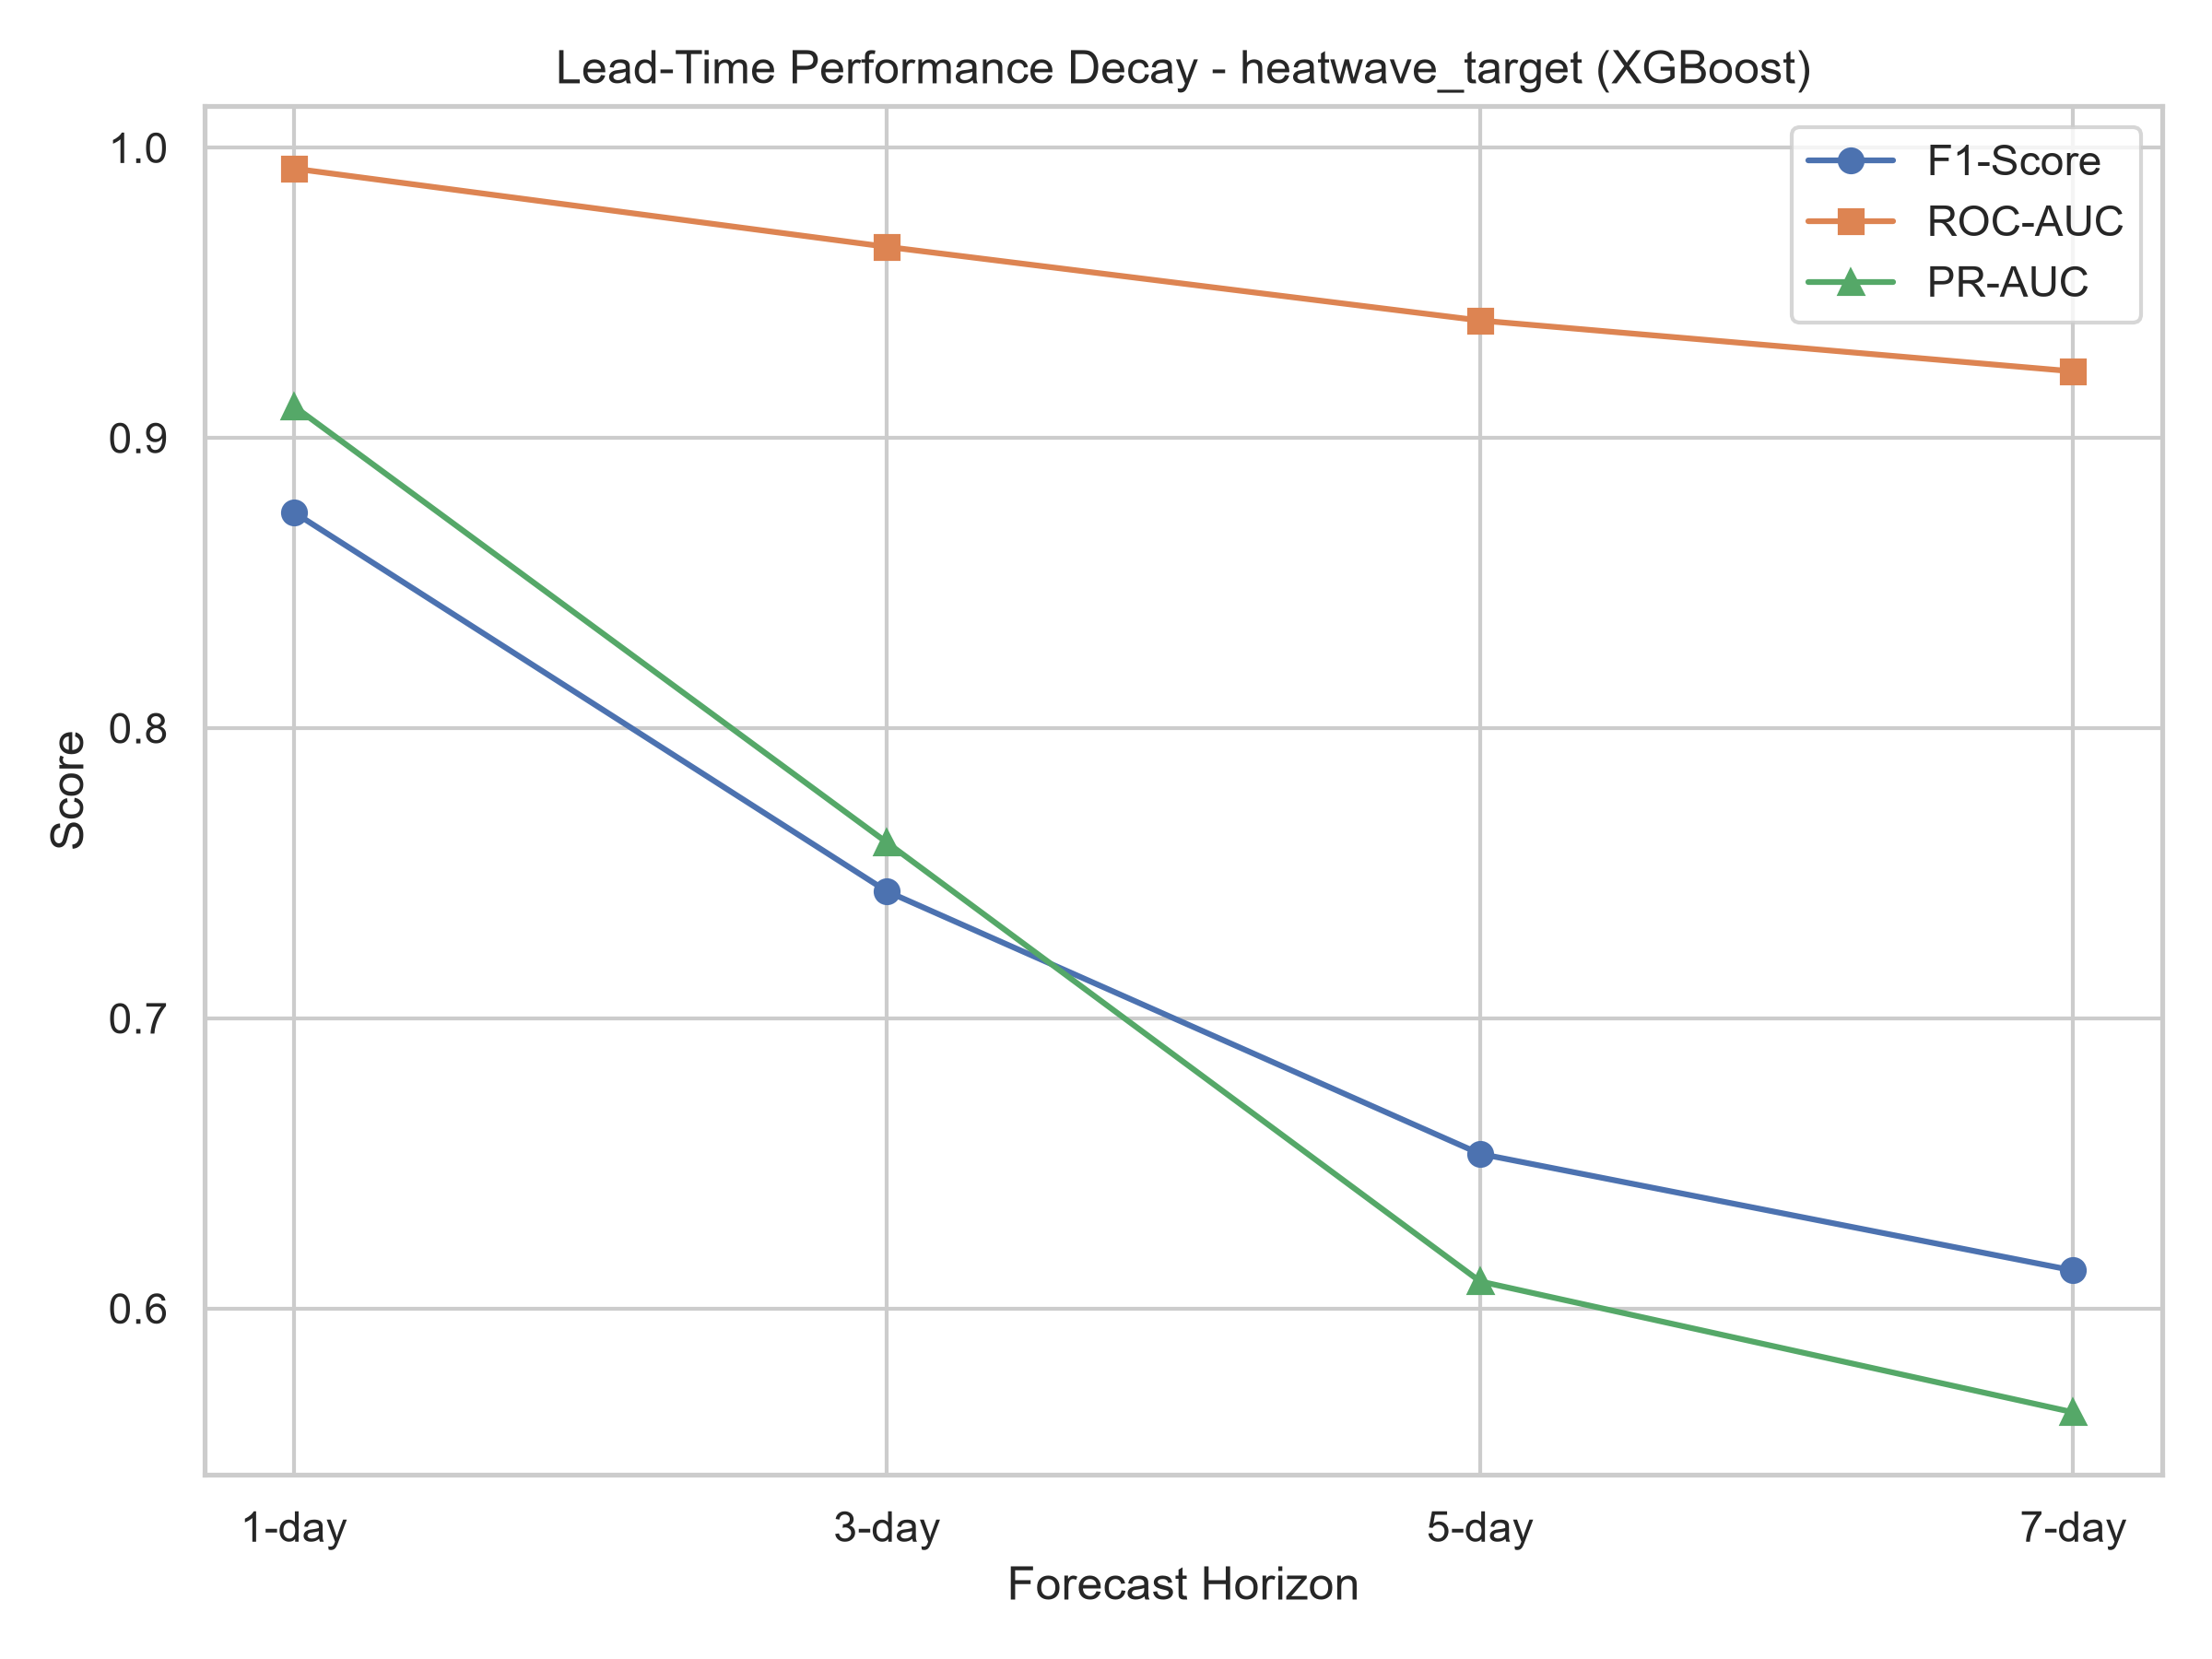
\includegraphics[width=\columnwidth]{../Paper_Figures/Fig_04_Heatwave_LeadTime.png}
\caption{Heatwave prediction F1-score across verified lead-time horizons.}
\label{fig:heatwave_leadtime}
\end{figure}
Establishing early-warning horizons is fundamentally necessary for operational deployment. Employing the heatwave target as an evaluation baseline (Fig.~\ref{fig:heatwave_leadtime}), the model's $F_1$-score degrades predictably as the horizon extends: 0.8744 at 1-day, 0.7437 at 3-days, and 0.6533 at 5-days. Importantly, the model retains significant discriminatory capacity through the 7-day horizon ($F_1=0.6131$), proving the viability of the engineered feature space for extended early-warning mechanisms.

\subsection{Ablation Study}
\begin{figure}[!t]
\centering
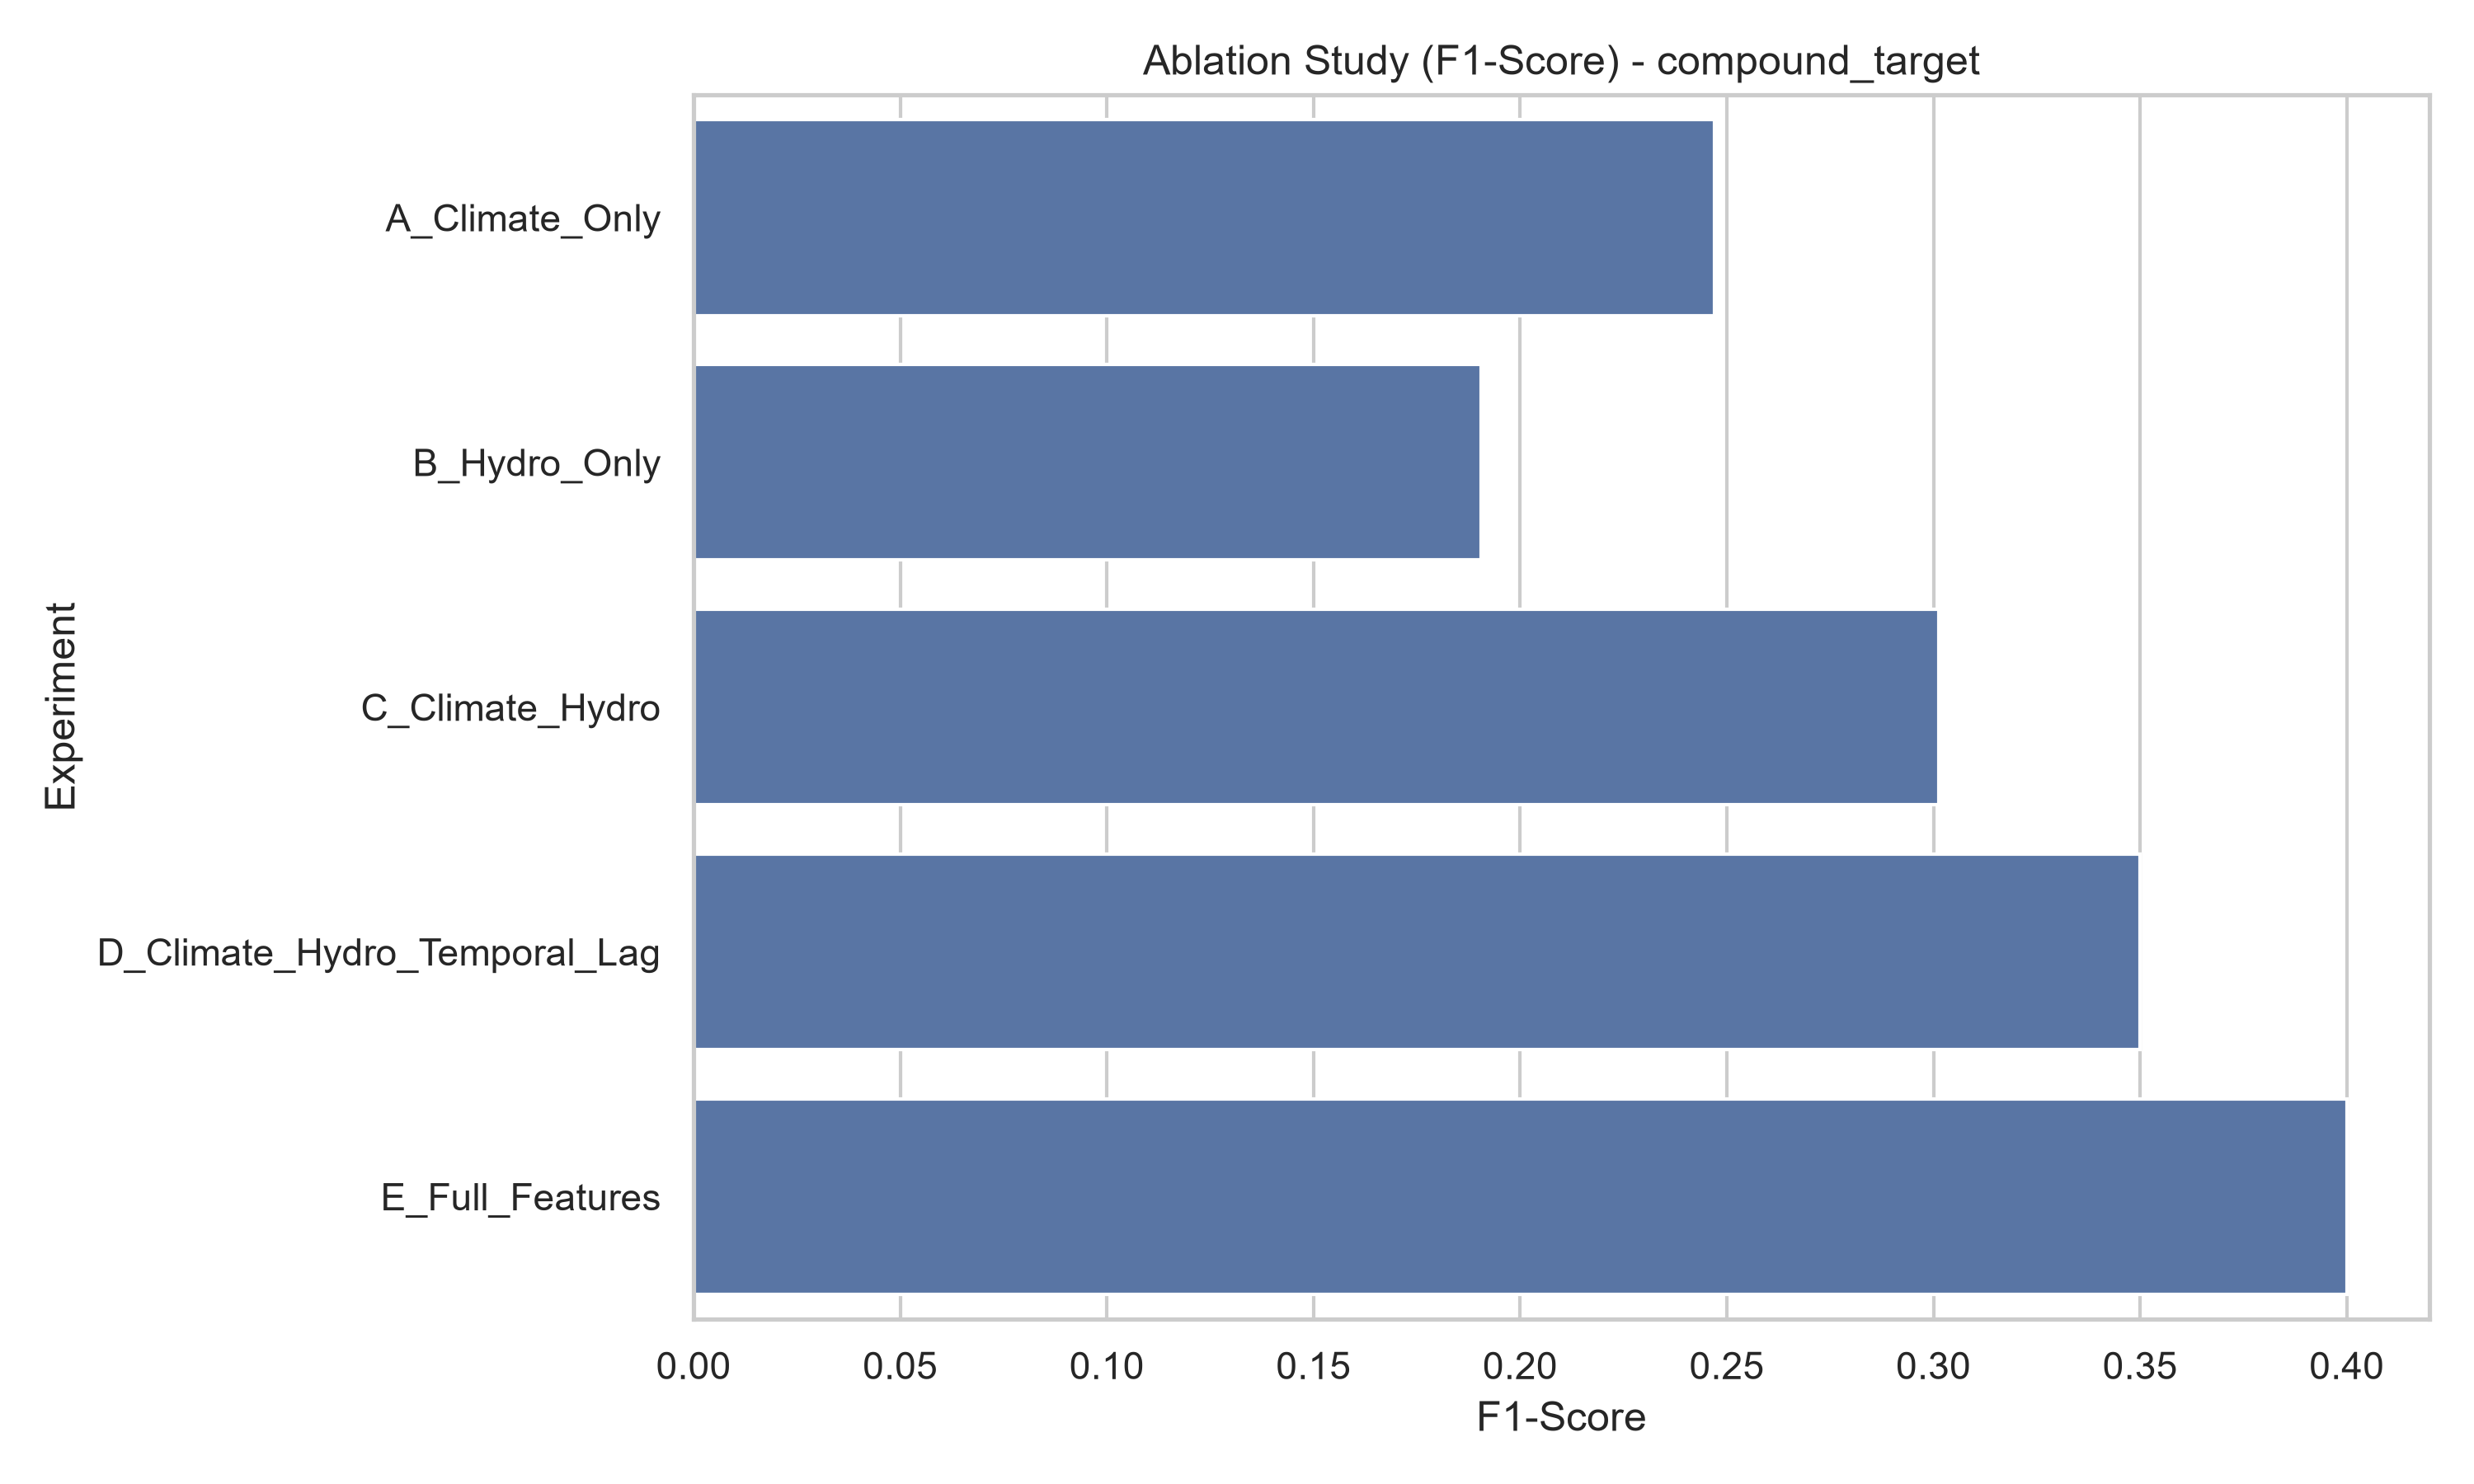
\includegraphics[width=\columnwidth]{../Paper_Figures/Fig_05_Compound_Ablation.png}
\caption{Compound-risk F1-score under the evaluated feature ablation configurations.}
\label{fig:compound_ablation}
\end{figure}

\begin{table}[htbp]
\caption{FEATURE ABLATION RESULTS FOR THE COMPOUND-RISK TARGET}
\begin{center}
\resizebox{\columnwidth}{!}{
\begin{tabular}{lc}
\toprule
\textbf{Feature Configuration} & \textbf{Compound F1-Score} \\
\midrule
Climate Only & 0.2469 \\
Hydro Only & 0.1905 \\
Climate + Hydro & 0.3014 \\
Climate + Hydro + Temporal/Lag & 0.3500 \\
Full Features & 0.4000 \\
\bottomrule
\end{tabular}
}
\label{tab:ablation}
\end{center}
\end{table}

Feature contribution was evaluated via an ablation protocol targeting the Compound hazard (Fig.~\ref{fig:compound_ablation} and Table~\ref{tab:ablation}). Isolated subspaces produced limited discrimination: Climate Only (0.2469) and Hydro Only (0.1905). Combining climate and hydrological features improved the F1-score to 0.3014. Reintegrating the engineered Temporal/Lag features further increased the F1-score to 0.3500, while the Full Features configuration achieved the highest observed F1-score of 0.4000.

\subsection{Probability Calibration}
\begin{figure}[!t]
\centering
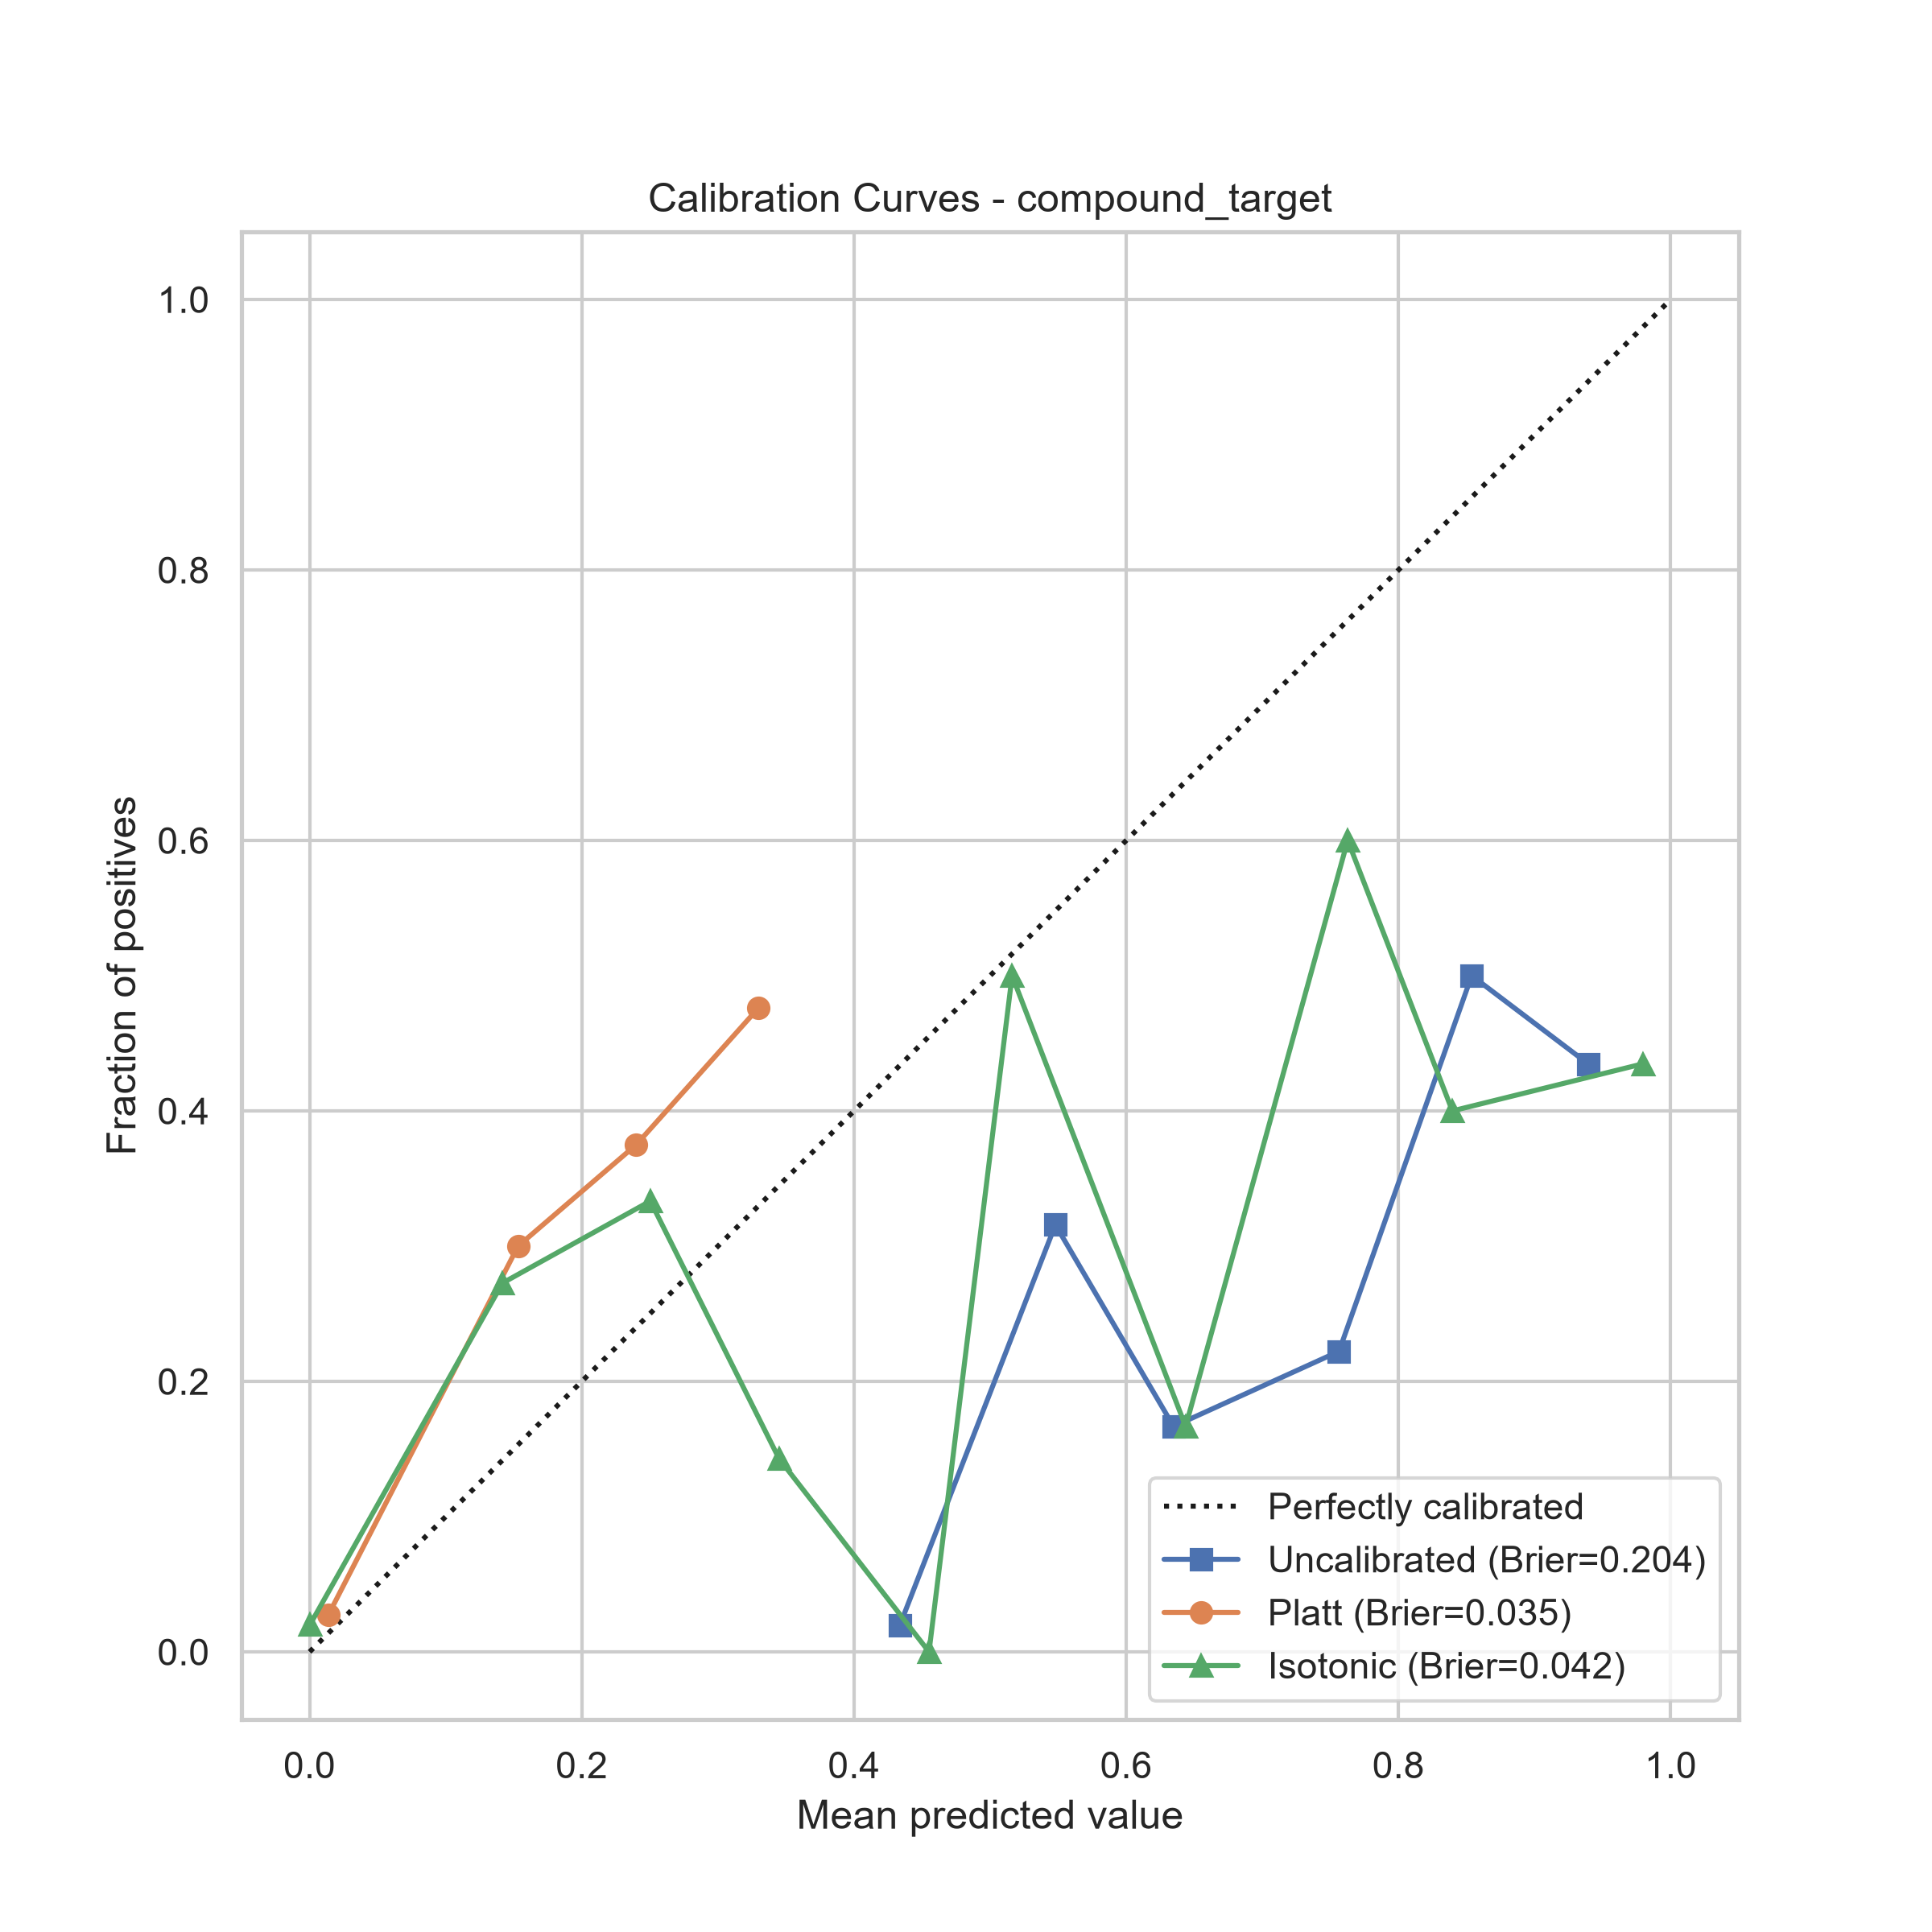
\includegraphics[width=\columnwidth]{../Paper_Figures/Fig_06_Compound_Calibration.png}
\caption{Brier-score comparison for uncalibrated, Platt-scaled, and isotonic-calibrated compound-risk probabilities.}
\label{fig:compound_calibration}
\end{figure}
Risk dissemination requires reliable probability values, not merely correct classification boundaries (Fig.~\ref{fig:compound_calibration}). Comparing outputs against the uncalibrated Compound model baseline (Brier = 0.2039), post-processing via Platt Scaling \cite{Platt1999} substantially rectified interval reliability (Brier = 0.0347), marginally outperforming Isotonic Regression \cite{Zadrozny2002} (Brier = 0.0415).

\subsection{SHAP-Based Interpretation}
\begin{figure}[!t]
\centering
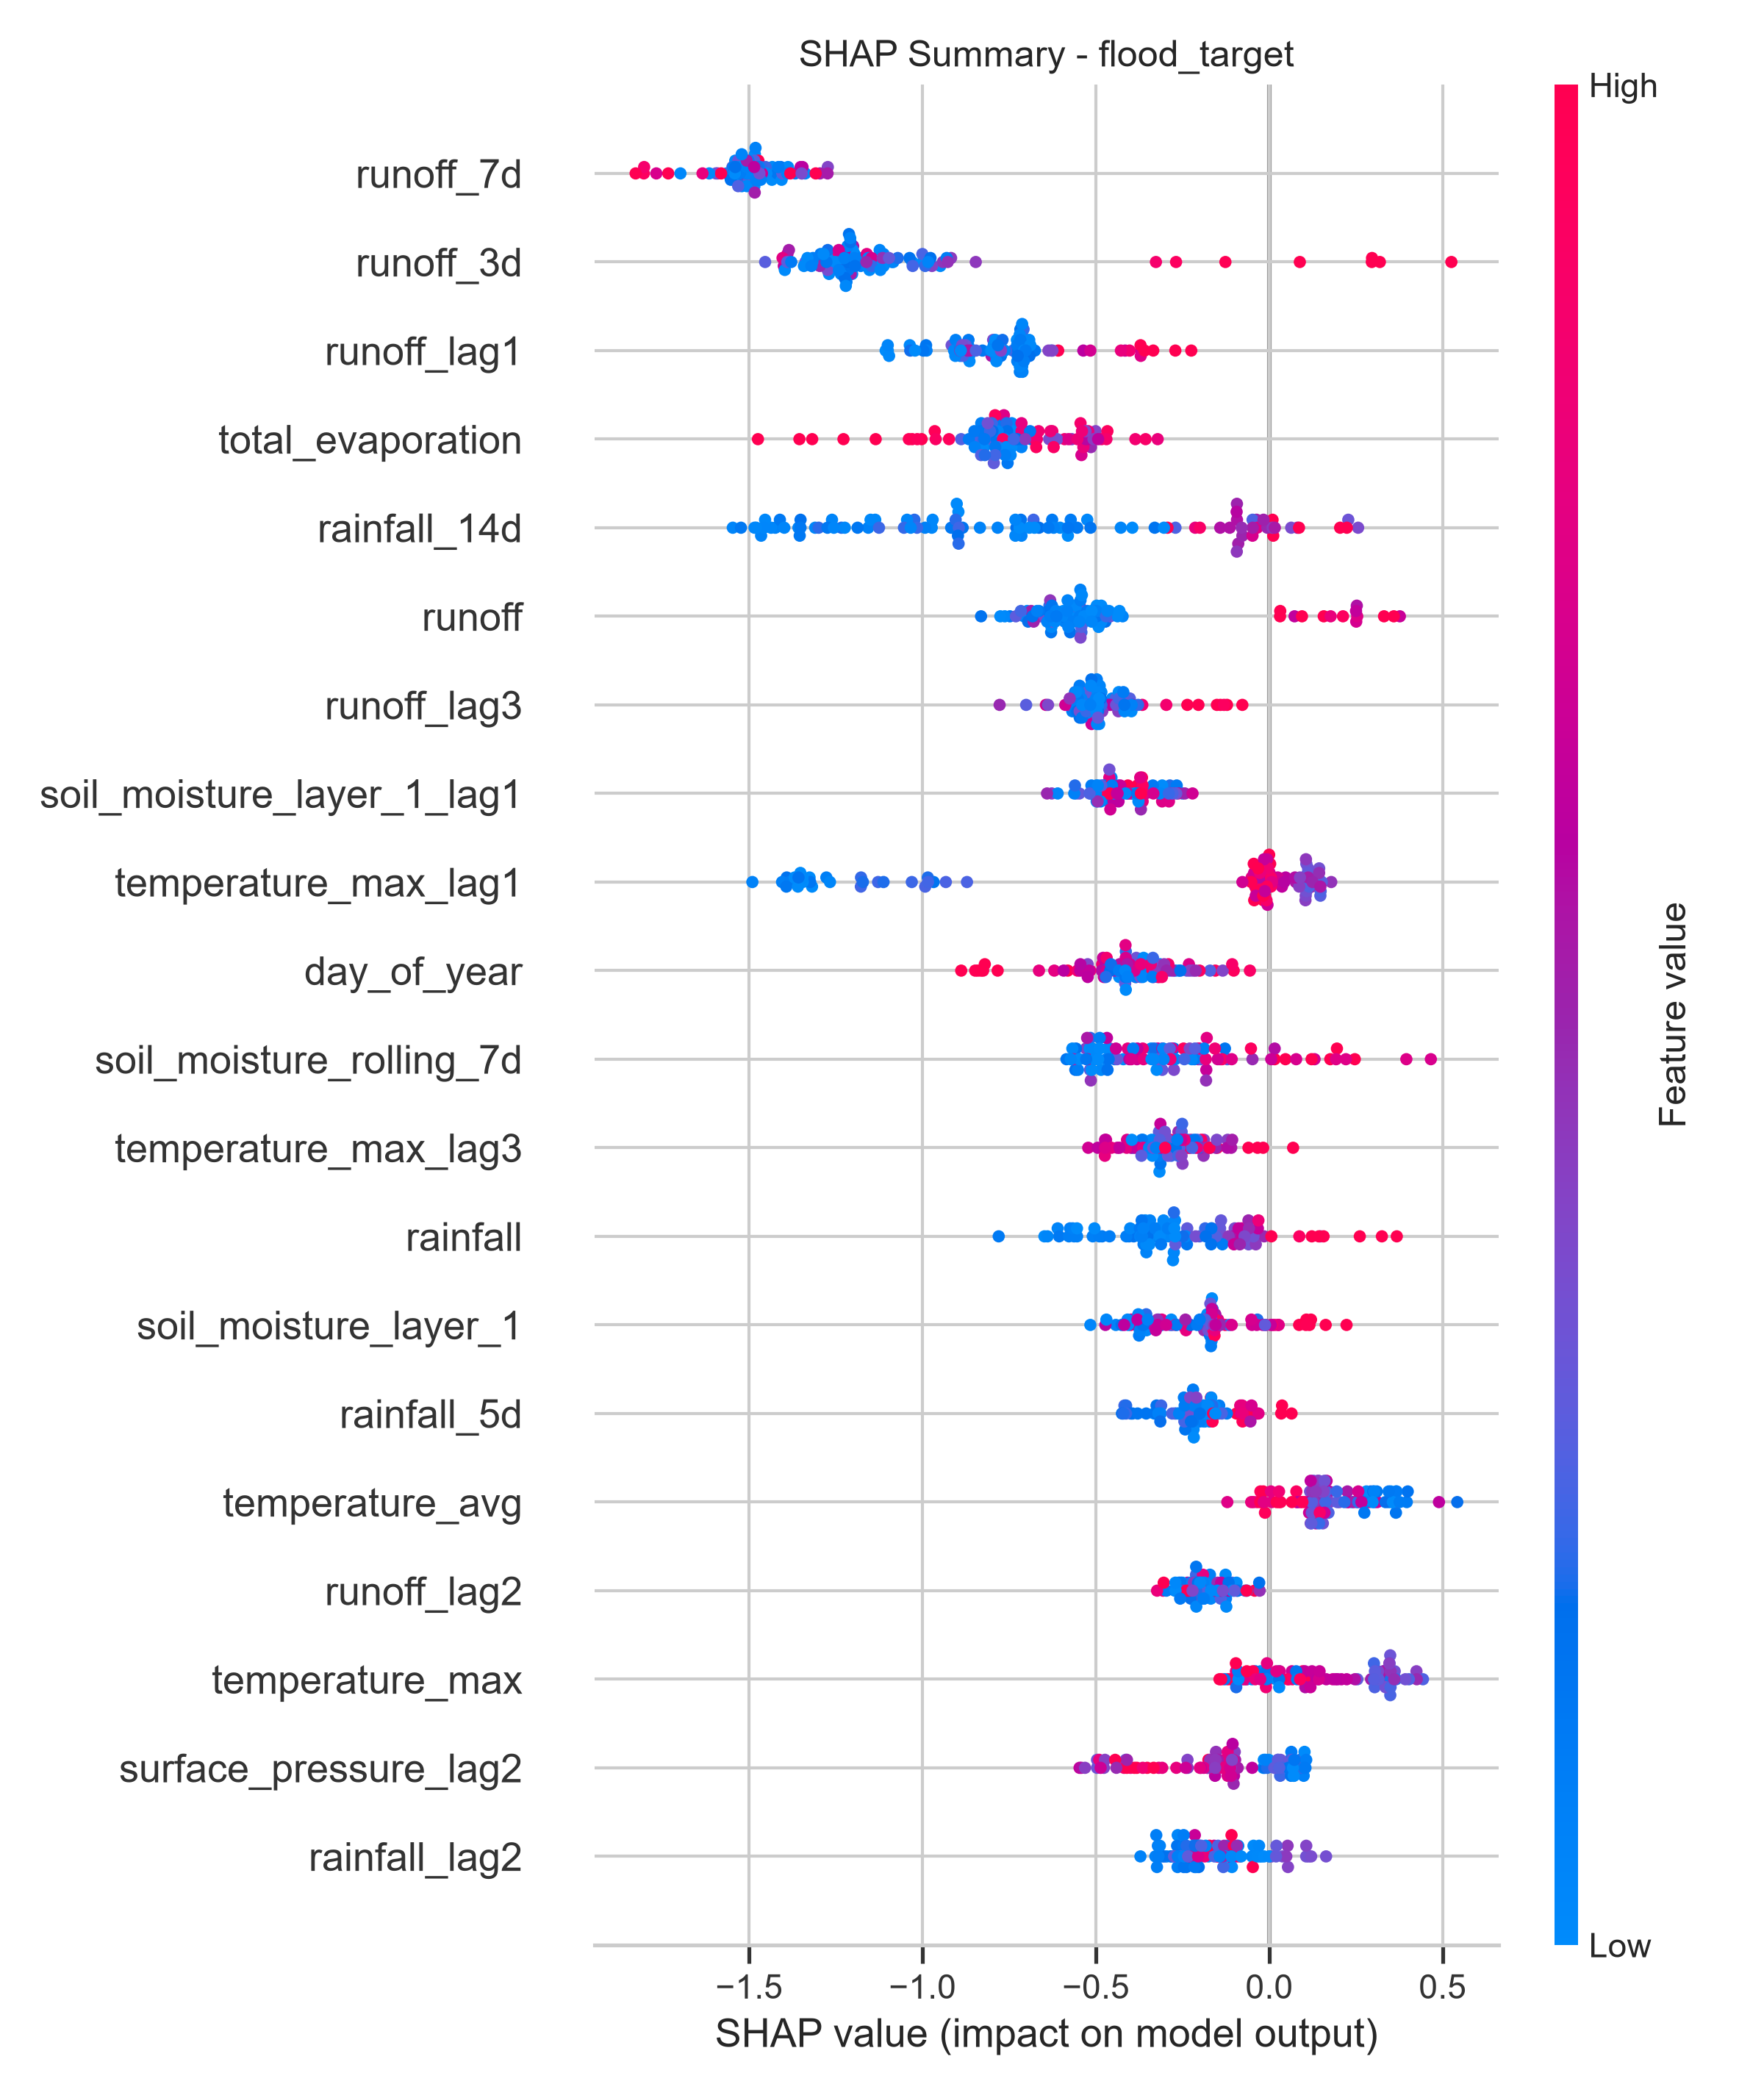
\includegraphics[width=\columnwidth]{../Paper_Figures/Fig_07_Flood_SHAP.png}
\caption{SHAP-based feature importance for model interpretation.}
\label{fig:flood_shap}
\end{figure}
To satisfy explainability mandates, the internal structural dependencies of the evaluated algorithms were mapped utilizing SHAP (SHapley Additive exPlanations) \cite{Lundberg2017}. Applied to the Flood model (Fig.~\ref{fig:flood_shap}), SHAP definitively ranks specific localized precipitation accumulation parameters as primary indicators governing positive classification. These attributions provide vital transparency into the machine learning algorithm's specific boundary construction without asserting fundamental physical causation.
